\documentclass{article}
\usepackage{amsmath}
\usepackage{amssymb}
\usepackage{graphicx}
\usepackage{enumitem}
\usepackage[utf8]{inputenc}
\usepackage{xcolor}


\graphicspath{{/home/stephanie/Escritorio/THC/Taller-de-Herramientas-Computacionales/Clases/Latex/Imagenes/}}

\title{\Huge Taller de Herramientas Computacionales}
\author{Stephanie Escobar Sánchez}
\date{23/enero/2019}


\begin{document}
	\maketitle
	\begin{center}
		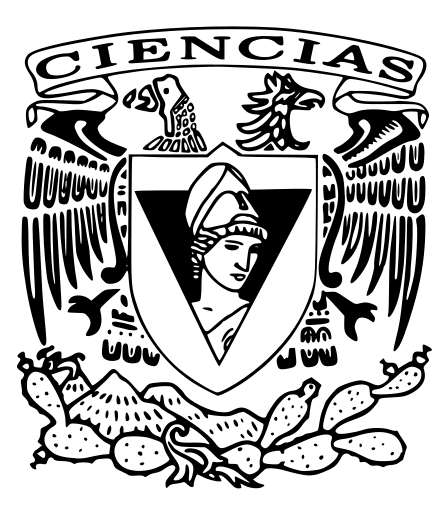
\includegraphics[scale=0.40]{1.png}	
	\end{center}
	\newpage
	\begin{center}
		\title {\Huge Problema 6} 
	\end{center}

\textit{Calcular el promedio de 10 datos}\\
\\
Primero fue fácil debido a que unicamente se metieron las variables de los 10 datos y finalmente eso entre 10, así solo era necesario asignar las variables y sacar el promedio.\\
\\
\section*{Listas}
Para las listas en este problema ya se pudo modificar el código de tal manera que no solo funcionara para 10 datos sino para todos los posibles, se creó una lista vacía en la que se asignaran los valores que el usuario da y eso dividido entre n, en este caso las listas lo facilitaron.

\end{document}